\documentclass{standalone}

\usepackage{tikz}

\begin{document}
    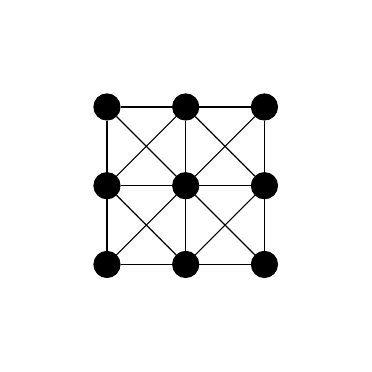
\begin{tikzpicture}
        \phantom{\draw (-1,-1) rectangle (3,3);}
        \foreach \i in {0,1,2}{
            \foreach \j in {0,1,2}{
                \node[draw,circle,fill=black] (\i\j) at (\i,\j) {};
            }
        }
        \foreach \a/\b in {00/01,00/10,00/11,01/02,01/10,01/11,01/12,02/11,02/12,10/11,10/20,10/21,11/12,11/20,11/21,11/22,12/21,12/22,20/21,21/22}{
            \draw (\a) -- (\b);
        }

%        \foreach \a/\b in {00/01,01/10,12/21,21/20}{
%            \draw[ultra thick] (\a) -- (\b);
%        }
        
    \end{tikzpicture}
\end{document}